% Kopfzeile beim Kapitelanfang:
\fancypagestyle{plain}{
%Kopfzeile links bzw. innen
\fancyhead[L]{\Large Vorlesung 16 (05.12.2013)}
%Kopfzeile rechts bzw. außen
\fancyhead[R]{}}
%Kopfzeile links bzw. innen
\fancyhead[L]{\Large Vorlesung 16 (05.12.2013)}
%Kopfzeile rechts bzw. außen
\fancyhead[R]{}
% **************************************************
\begin{tikzpicture}
\draw (0,0)--(3,0);
\draw (1.5,0) node[below] {$b$};
\draw (3,0)--(3,3);
\draw (3,1.5) node[right] {$c$};
\draw (0,0)--(3,3);
\draw (1.3,1.5) node[left] {$a$};
\draw (0.5,0) arc (0:45:0.5);
\draw (0.8,0.3) node {$\varphi$};
\draw (3,0.5) arc (90:180:0.5);
\draw (2.8,0.2) node {$\cdot$};
\end{tikzpicture}\nl
$cos \ \varphi := \frac{b}{a}$ und $sin \ \varphi := \frac{c}{a}$\\
$cos \ x = \sum_{k=0}^\infty \frac{(-1)^k}{(2k)!} x^{2k} = 1 - \frac{x^2}{2} + \frac{x^4}{24} \mp \ldots$\\
$sin \ x = \sum_{k=0}^\infty \frac{(-1)^k}{(2k+1)!} x^{2k+1} = x - \frac{x^3}{3!} + \frac{x^5}{5!} \mp \ldots$\nl
\textbf{Problem}: Wir wissen nicht, was ein Winkel ist.

\subsection*{Beweis von \ref{8.20}}
\en{
\item $x=0$: \ok\\
$x \neq 0$: $cos \ x = \sum_{k=0}^\infty (-1)^k \underbrace{\frac{x^{2k}}{(2k)!}}_{a_k > 0}$\\
$\frac{a_{k+1}}{a_k} = \frac{x^2}{(2k+2)(2k+1)} \le \frac{4}{(2k+2)(2k+1)} < 1$ für $k \ge 1$\\
$\Ra (a_k)_{k \ge 1}$ ist monoton fallende Nullfolge und die Cosinus-Reihe konvergiert.\\
Leibniz-Kriterium (\ref{7.8}) $\Ra cos \ x$ liegt zwischen je zwei aufeinanderfolgenden Partialsummen $\Ra$ Behauptung
\item In der Übung.
} \qed

\chapter{Stetige Funktionen und Grenzwerte}\label{P9}
Sei $D \subseteq \R, f: D \to \R$ eine Funktion mit $D$ als Definitionsbereich.\\
Varianten: \\
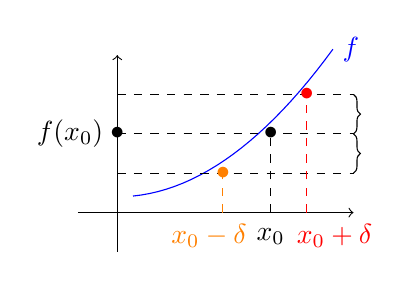
\begin{tikzpicture}
\draw[->] (-0.5,0)--(3,0);
\draw[->] (0,-0.5)--(0,2);
\draw[blue, domain=0.2:2.73861] plot (\x, {0.25*\x^2+0.2}) node [right] {$f$};
\draw[dashed] (0,0.5)--(3,0.5);
\draw[dashed] (0,1)--(3,1);
\draw (0,1) node {$\bullet$};
\draw (-0.6,1) node {$f(x_0)$};
\draw[dashed] (0,1.5)--(3,1.5);
\draw [decoration={brace,mirror,raise=0.5cm},decorate] (2.5,0.5)--(2.5,1);
\draw (3.3,0.75) node {$\eps$};
\draw [decoration={brace,mirror,raise=0.5cm},decorate] (2.5,1)--(2.5,1.5);
\draw (3.3,1.25) node {$\eps$};
\draw[color=orange,dashed] (1.3416408,0)--(1.3416408,0.5);
\draw[color=orange] (1.3416408,-0.3) node {$x_0-\delta \ \ \ $};
\draw[color=orange] (1.3416408,0.5) node {$\bullet$};
\draw[dashed] (1.9493589,0)--(1.9493589,1);
\draw (1.9493589,-0.3) node {$x_0$};
\draw (1.9493589,1) node {$\bullet$};
\draw[color=red,dashed] (2.4083189,0)--(2.4083189,1.5);
\draw[color=red] (2.4083189,-0.3) node {$\ \ \ \ \ \ x_0+\delta$};
\draw[color=red] (2.4083189,1.5) node {$\bullet$};
\end{tikzpicture} \ 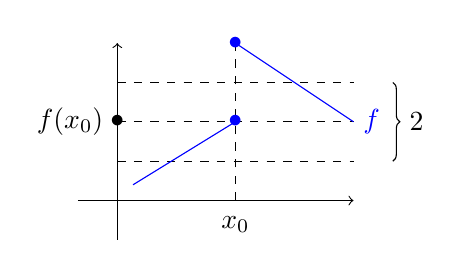
\begin{tikzpicture}
\draw[->] (-0.5,0)--(3,0);
\draw[->] (0,-0.5)--(0,2);
\draw[dashed] (0,0.5)--(3,0.5);
\draw[dashed] (0,1)--(3,1);
\draw (0,1) node {$\bullet$};
\draw (-0.6,1) node {$f(x_0)$};
\draw[dashed] (0,1.5)--(3,1.5);
\draw[dashed] (1.5,0)--(1.5,2);
\draw (1.5,-0.3) node {$x_0$};
\draw[color=blue] (0.2,0.2)--(1.5,1);
\draw[color=blue] (1.5,1) node {$\bullet$};
\draw[color=blue] (1.5,2)--(3,1) node[right] {$f$};
\draw[color=blue] (1.5,2) node {$\bullet$};
\draw [decoration={brace,mirror,raise=0.5cm},decorate] (3,0.5)--(3,1.5);
\draw (3.8,1) node {$2\eps$};
\end{tikzpicture}\nl
Anschaulich: $f$ ist stetig in $x_0 :\Lra f$ hat keinen Sprung in $x_0$.\nl
Mathematisch präzise Fassung:

\section{\texorpdfstring{Definition: $\eps$-$\delta$-Kriterium}{Definition: Epsilon-Delta-Kriterium}}\label{9.1}
Sei $D \subseteq \R, f: D \to \R$ eine Funktion.\\
$f$ heißt \underline{stetig} in $x_0 \in D :\Lra$
$$\forall \eps > 0 \exists \delta > 0: |f(x)-f(x_0)| < \eps \text{ für alle } x \in D \text{ mit } |x-x_0| < \delta$$
$f$ stetig auf $D :\Lra f$ stetig in jedem $x_0 \in D$.\\
Interpretation: $x \rightarrow$ {\fbox{$\underset{\text{Programm}}{f}$} $\rightarrow f(x)$\\
Kleine Änderungen der Eingaben bewirken nur kleine Änderungen der Ausgabe.

\subsection*{Beispiele}
\en{
\item $f: \R \to \R, f(x)=ax+b$ ($a,b \in \R$)\nl
$f$ ist stetig auf ganz $\R$, denn:\\
Sei $x_0 \in \R \Ra |f(x)-f(x_0)| = |a| \cdot |x-x_0|$\\
\items{
\item[1. Fall] $a=0 \Ra |f(x)-f(x_0)| = 0$\\
Wähle $\delta = 1$ (zu vorgeg. $\eps > 0$)
\item[2. Fall] $a \neq 0$. Sei $\eps > 0$ vorgegeben.\\
$\delta := \frac{\eps}{|a|} \Ra |f(x)-f(x_0)| < \eps \forall x \in \R$ mit $|x-x_0| < \delta$
}
\newpage
\item \underline{Heaviside-Funktion}: $H: \R \to \R$\\
$H(x) = \left\{\begin{array}{l l} 1 & \text{falls } x \ge 0 \\ 0 & \text{falls } x < 0 \end{array}\right.$\\
\begin{tikzpicture}
\draw[->] (-2,0)--(2,0);
\draw[->] (0,-0.5)--(0,2);
\draw[thick,color=blue] (-2,0)--(0,0);
\draw (-0.2,-0.2) node {$0$};
\draw[thick,color=blue] (0,1)--(2,1);
\draw (-0.2,1) node {$1$};
\draw[color=blue] (0,0) node {$\bullet$};
\draw[color=blue] (0,1) node {$\bullet$};
\draw[dashed] (-2,0.5)--(2,0.5);
\draw[dashed] (-2,1.5)--(2,1.5);
\draw [decoration={brace,mirror,raise=0.5cm},decorate] (1.6,0.5)--(1.6,1);
\draw (2.4,0.75) node {$\frac{1}{2}$};
\end{tikzpicture}\\
$H$ ist unstetig in $x_0 = 0$\\
Denn: $x < 0$ bel. $\Ra |\overbrace{H(x)}^{=0} - \overbrace{H(0)}^{=1}| = 1$\nl
Wähle $\eps := \frac{1}{2} \Ra \nexists \delta > 0$ so, dass das $\eps$-$\delta$-Kriterium (\ref{9.1}) in $x_0=0$ erfüllt ist!\\
Aber: $H$ stetig auf $\R \setminus \{0\}$
}
Wichtiges Kriterium:

\section{Folgenkriterium für Stetigkeit reeller Funktionen}\label{9.2}
Für $f: D \to \R$ gilt:\\
$f$ ist stetig in $x_0 \in D :\Lra$ für jede Folge $(x_n) \subseteq D$ mit $x_n \to x_0$ gilt: $\lim_{n \to \infty} f(x_n) = f(x_0)$\nl
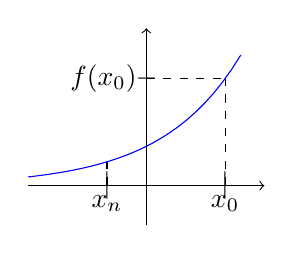
\begin{tikzpicture} [domain=-3:3]
\draw[->] (-1.5,0)--(1.5,0);
\draw[->] (0,-0.5)--(0,2);
\draw[blue, domain=-1.5:1.2] plot (\x, {0.5*exp(\x)});
\draw[dashed] (1,0)--(1,1.3591409);
\draw[dashed] (0,1.3591409)--(1,1.3591409);
\draw (0,1.3591409) node{$-$} [left] node{$f(x_0)$};
\draw (-0.5,0) node {$|$} [below] node {$x_n$};
\draw[dashed] (-0.5,0)--(-0.5,0.303265329856);
\draw (1,0) node{$|$} [below] node{$x_0$};
\end{tikzpicture}\nl
$\eps$-$\delta$-Definition der Stetigkeit in $x_0$:
$$\forall \eps > 0 \exists \delta > 0: |f(x)-f(x_0)| < \eps \forall x \in D \text{ mit } |x-x_0| < \delta$$

\subsection*{Beweis}
\items{
\item[``$\Ra$''] Sei $(x_n) \subseteq D$ mit $x_n \to x_0$.\\
Sei $\eps > 0 \overset{\text{\ref{9.1}}}{\Ra} \exists \delta > 0:$\\
$|f(x_n)-f(x_0)| < \eps$, sofern $|x_n-x_0| < \delta$.\\
$\lim_{n \to \infty} x_n = x_0 \Ra \exists n_0 \in \N: |x_n-x_0| < \delta \forall n \ge n_0$\\
Also: $|f(x_n)-f(x_0)| < \eps \forall n \ge n_0 \Ra f(x_n) \to f(x_0)$
\item[``$\La$''] Angenommen, $f$ sei unstetig in $x_0$.\\
Dann $\exists \eps_0 > 0$, zu dem sich kein $\delta$ finden lässt, so dass das $\eps$-$\delta$-Kriterium (\ref{9.1}) erfüllt ist.\\
Insbes.: Zu $\frac{1}{n} = \delta$ ($n \in \N$) $\exists x_n \in D:$\\
$|x_n-x_0| < \frac{1}{n}$, aber $|f(x_n)-f(x_0| \ge \eps_0$. Also: $x_n \to x_0$, aber $f(x_n) \nrightarrow f(x_0)$ \wspruch
} \qed

\newpage

\subsection*{Beispiele}
\en{
\item $f(x)=\frac{1}{x}$ ist stetig auf $D = \R \setminus \{0\}$.\nl
\begin{tikzpicture}
\draw[->] (-2,0)--(2,0);
\draw[->] (0,-2)--(0,2);
\draw (-0.2,-0.2) node {$0$};
\draw[color=blue,domain=-2:-0.5] plot (\x, {1/\x});
\draw[color=blue,domain=0.5:2] plot (\x, {1/\x});
\end{tikzpicture}\nl
Denn: Sei $x_0 \neq 0, (x_n) \subseteq \R \setminus \{0\}$ Folge mit $x_n \to x_0$\\
$\Ra f(x_n) = \frac{1}{x_n} \to \frac{1}{x_0} = f(x_0)$
\item $f(x)=|x|$ ist stetig auf $\R$.\nl
\begin{tikzpicture}
\draw[->] (-2,0)--(2,0);
\draw[->] (0,-0.5)--(0,2);
\draw (-0.2,-0.2) node {$0$};
\draw[color=blue,domain=-2:2] plot (\x, {abs(\x)});
\end{tikzpicture}\nl
Denn: $x_n \to x_0 \Ra |x_n| \to |x_0|$
}

\section{Regeln für stetige Funktionen}\label{9.3}
Seien $f,g: D \to \R$ stetig in $x_0 \in D \Ra$
$$f+g, f \cdot g, c \cdot f (c \in \R): D \to \R$$
sind ebenfalls stetig in $x_0$.\\
(Dabei: $(f \underset{\cdot}{+} g)(x)=f(x) \underset{\cdot}{+} g(x), (c \cdot f)(x) = c \cdot f(x)$)\\
Falls $g(x_0) \neq 0 \Ra \frac{f}{g}: \{x \in D: g(x) \neq 0\} \to \R$ ist stetig in $x_0$

\subsection*{Beweis}
Mit Folgenkriterium (\ref{9.2}) und Regeln für Grenzwerte (\ref{6.18}):\\
Sei $(x_n) \subseteq D$ mit $x_n \to x_0$\\
$\Ra f(x_n) \to f(x_0), g(x_n) \to g(x_0)$\\
$\Ra f(x_n)+g(x_n) \to f(x_0)+g(x_0) \Ra f+g$ stetig in $x_0$, etc.\nl
Zu $\frac{f}{g}$: $\underbrace{g(x_0)}_{=: c} \neq 0 \underset{g \text{ stetig in } x_0}{\Ra} \exists n_0 \in \N: |g(x_n)| > \frac{1}{2} c > 0 \forall n \ge n_0$\\
$\Ra \frac{f(x_n)}{g(x_n)} \to \frac{f(x_0)}{g(x_0)}$

\newpage

\section{Beispiele: Polynome und rationale Funktionen}\label{9.4}
\en{
\item Sei $p(x) = a_n x^n + \ldots + a_1 x + a_0 \in \Pow_\R$ eine Polynomfunktion.\\
Wiederholte Anwendung von \ref{9.3} $\Ra p$ ist stetig auf $\R$.
\item Eine \underline{rationale Funktion} auf $\R$ ist eine Funktion der Form $R(x) = \frac{p(x)}{q(x)}$ mit $p,q \in \Pow_\R, q \neq 0$ (Nullpolynom).\\
Definitionsbereich: $D = \{x \in \R: q(x) \neq 0\}$ (höchstens endlich viele Def.-Lücken!)\\
Regeln \ref{9.3} $\Ra R$ stetig auf ganz $D$\nl
Vergrößerung von $D$ eventuell möglich durch Kürzen gemeinsamer Faktoren.\\
Beispiel: $R(x) = \frac{x}{x^3-x} = \frac{1}{x^2-1}$ stetig auf $\R \setminus \{\pm 1\} = D_{\text{max}}$
}

\section{Satz}\label{9.5}
$exp: \R \to \R, x \mto e^x$ ist stetig auf $\R$.

\subsection*{Beweis}
\en{
\item $exp$ ist stetig in $x_0=0$, denn:\\
Sei $x_n \to 0 \Ra |e^{x_n} - e^0| = |e^{x_n}-1| \underset{\text{für } |x_n \le 1}{\le} 2|x_n| \overset{n \to \infty}{\to} 0$\\
$\Ra \lim_{n \to \infty} e^{x_n} = e^0$
\item $exp$ ist stetig in jedem $x_0 \in \R$, denn:\\
Sei $x_n \to x_0 \Ra |e^{x_n}-e^{x_0}| = |e^{x_0} (e^{x_n-x_0} -1)| = |e^{x_0}| \cdot \underbrace{|e^{x_n-x_0}-e^0|}_{\to 0 \text{ nach 1.}}$\\
$\Ra \lim_{n \to \infty} |e^{x_n} - e^{x_0}| = 0$
} \qed

\section{Komposition stetiger Funktionen}\label{9.6}
Seien $D,E \subseteq \R$ und $f: D \to \R, g: E \to \R$ Funktionen mit $f(D) \subseteq E$.\\
$f$ sei stetig in $x_0 \in D$, $g$ stetig in $f(x_0) \in E \Ra$\\
$g \circ f: D \to \R$ ist stetig in $x_0$

\subsection*{Beweis}
Sei $(x_n) \subseteq D, x_n \to x_0 \overset{f \text{ stetig}}{\Ra} f(x_n) \to f(x_0) \overset{g \text{ stetig}}{\Ra} g(f(x_n)) \to g(f(x_0))$ \qed

\subsection*{Beispiel}
\en{
\item $f(x) = e^{x^2} = e^{(x^2)}$ stetig auf $\R$.
\item $f: D \to \R$ stetig $\Ra |f|: D \to \R$, $|f|(x)=|f(x)|$ stetig auf $D$, da $|f| = |.| \circ f$
}